\documentclass[../main.tex]{subfiles}
\begin{document}
%=========================================================
% TĐ_PBT_IQA_HK1_Tuan17_OnTapPhepNhan_BaiToanCoLoiVan
% Phiếu bài tập Toán tư duy cấp độ A (lớp 2) - Ôn tập lần 3 (Buổi 1) và lần 4 (Buổi 2), mỗi buổi 90 phút
%   Buổi 1: ÔN TẬP PHÉP NHÂN (bảng nhân 2, bảng nhân 5)
%   Buổi 2: ÔN TẬP BÀI TOÁN CÓ LỜI VĂN (phép cộng, phép trừ trong phạm vi 100)
% Mỗi buổi chia 3 phần: A (khá) -> B (nâng cao) -> C (thử thách, dạng đề thi Toán quốc tế và trong nước)
% Soạn theo mẫu (\hktuan, bt, listEX). Không dùng hình ảnh ngoài: mọi hình đều vẽ bằng TikZ.
% Đáp án và hướng dẫn giải: xem file DapAn_Tuan_17_OnTapPhepNhan_BaiToanCoLoiVan.tex
%=========================================================

%---------- Lệnh dùng riêng cho phiếu ----------
% Chỗ chấm điền
\providecommand{\TTcham}[1][3cm]{\makebox[#1]{\dotfill}}
% Ô vuông trống để điền số hoặc dấu
\providecommand{\TTdien}[1][0.9cm]{\framebox[#1]{\rule{0pt}{0.62cm}}}
% Dòng thông tin học sinh
\providecommand{\TTthongtin}{%
  \noindent\begin{tabular}{|p{7.6cm}|p{4cm}|p{4cm}|}
    \hline
    \textbf{Họ và Tên HS:}\dotfill & \textbf{Lớp:}\dotfill & \textbf{Ngày:}\dotfill \\
    \hline
  \end{tabular}\par\medskip}
% Đánh lại số bài từ 1 cho buổi 2 (chỉ khi môi trường bt có bộ đếm tên bt)
\makeatletter
\providecommand{\TTdatlaibai}{\@ifundefined{c@bt}{}{\setcounter{bt}{0}}}
\makeatother
% Bắt đầu phần hình vẽ TikZ ngay dưới đề bài
\providecommand{\TTbatdauhinh}{}\renewcommand{\TTbatdauhinh}{\par\nopagebreak\vspace{4pt}\nopagebreak}
% Ngôi sao mức độ: \TTsao{số sao}
\providecommand{\TTsao}{}\renewcommand{\TTsao}[1]{\foreach \s in {1,...,#1}{$\bigstar$}}
% Tiêu đề từng phần A, B, C trong khung: \TTphan{chữ cái}{tên phần}{số sao}
\providecommand{\TTphan}{}\renewcommand{\TTphan}[3]{%
  \par\medskip\noindent
  \begin{tcolorbox}[colback=mauchinh!8,colframe=mauchinh,boxrule=0.7pt,arc=3pt,left=6pt,right=6pt,top=3pt,bottom=3pt]
    {\color{mauchinh}\bfseries PHẦN #1.\ #2}\hfill{\color{orange!85!black}\TTsao{#3}}
  \end{tcolorbox}\par\nopagebreak\vspace{2pt}}
% Nhãn nguồn của bài thử thách: \TTnguon{Dạng đề Kangaroo}
\providecommand{\TTnguon}{}\renewcommand{\TTnguon}[1]{\textit{\small\color{red!70!black}[#1]}\ }
% Khung ghi nhớ / gợi ý nhỏ
\providecommand{\TTgoiy}{}\renewcommand{\TTgoiy}[1]{%
  \par\smallskip\noindent\begin{tcolorbox}[colback=yellow!12,colframe=orange!70,boxrule=0.5pt,arc=2pt,left=5pt,right=5pt,top=2pt,bottom=2pt]\small #1\end{tcolorbox}\par}

% ---- Trình bày bài giải theo mẫu lớp 2 ----
% \TTgiai{số bước}: "Bài giải" + mỗi bước gồm 1 dòng câu lời giải và 1 dòng phép tính (đơn vị), cuối cùng là dòng Đáp số.
% Bài 1 bước tính -> \TTgiai{1} (2 dòng kẻ); bài 2 bước tính -> \TTgiai{2} (4 dòng kẻ); bài 3 bước tính -> \TTgiai{3} (6 dòng kẻ).
\providecommand{\TTgiai}{}\renewcommand{\TTgiai}[1]{%
  \par\smallskip\noindent\textbf{Bài giải}%
  \foreach \b in {1,...,#1}{\par\vspace{7pt}\noindent\dotfill\par\vspace{7pt}\noindent\hspace*{1.2cm}\TTcham[5cm]\,=\,\TTcham[2cm]\ (\TTcham[1.8cm])}%
  \par\vspace{7pt}\noindent\textbf{Đáp số:}\ \TTcham[2.5cm]\ \TTcham[4.5cm]\par\smallskip}
% \TTnhap{số dòng}: dòng kẻ để học sinh tự trình bày cách làm (bài thử thách không theo mẫu cố định)
\providecommand{\TTnhap}{}\renewcommand{\TTnhap}[1]{%
  \par\smallskip\noindent\textbf{Cách làm:}\ \dotfill\foreach \d in {2,...,#1}{\par\vspace{9pt}\noindent\dotfill}\par\vspace{4pt}}
% Dòng đáp số tự do
\providecommand{\TTdapso}{}\renewcommand{\TTdapso}{\par\vspace{4pt}\noindent\textbf{Đáp số:}\ \TTcham[6cm]\par\smallskip}
% \TTviettt{số dòng}: dòng kẻ để học sinh tự viết tóm tắt
\providecommand{\TTviettt}{}\renewcommand{\TTviettt}[1]{%
  \par\smallskip\noindent\textbf{Tóm tắt}\foreach \d in {1,...,#1}{\par\vspace{9pt}\noindent\hspace*{0.8cm}\TTcham[9cm]}\par\smallskip}
% \TTtomtat{dòng 1}{dòng 2}: tóm tắt cho sẵn, mỗi dòng dạng "Mỗi đĩa: & 5 quả cam"
\providecommand{\TTtomtat}{}\renewcommand{\TTtomtat}[2]{%
  \par\smallskip\noindent\textbf{Tóm tắt}\par\noindent\hspace*{0.8cm}\begin{tabular}{@{}l@{\quad}l@{}}#1\\ #2\end{tabular}\par\smallskip}
% Hộp đề toán dùng trong bài nối: \TTdeto{đề toán}
\tikzset{TTdeto/.style={anchor=west,text width=10.4cm,align=left,draw,rounded corners=3pt,inner sep=4pt,font=\small}}
\tikzset{TTpt/.style={draw,thick,rounded corners=3pt,minimum width=2.4cm,minimum height=0.8cm,font=\sffamily\large}}

%---------- Màu và hình vẽ TikZ ----------
\definecolor{TTxanh}{RGB}{100,180,240}\definecolor{TTxanhdam}{RGB}{30,110,200}
\definecolor{TTcam}{RGB}{255,185,90}\definecolor{TTcamdam}{RGB}{230,90,20}
\definecolor{TTdo}{RGB}{225,70,70}\definecolor{TTla}{RGB}{110,190,110}
\tikzset{
  TTochu/.style={draw,thick,rounded corners=3pt,minimum width=2.4cm,minimum height=0.72cm,inner sep=2pt,font=\sffamily\large},
}
% Một que diêm (từ điểm thứ nhất đến điểm thứ hai)
\providecommand{\TTque}{}\renewcommand{\TTque}[2]{\draw[line width=2.2pt,brown!70!black,line cap=round] #1--#2;\fill[red!80!black] #1 circle (2.2pt);}
% Hình vuông làm từ 4 que diêm, góc dưới trái tại (x,y), cạnh 1 đơn vị
\providecommand{\TThvque}{}\renewcommand{\TThvque}[2]{%
  \TTque{(#1,#2)}{(#1+1,#2)}\TTque{(#1+1,#2)}{(#1+1,#2+1)}\TTque{(#1+1,#2+1)}{(#1,#2+1)}\TTque{(#1,#2+1)}{(#1,#2)}}
% Quả cân: \TTcan{x}{y}{số ghi trên quả cân}{màu}
\providecommand{\TTcan}{}\renewcommand{\TTcan}[4]{%
  \draw[thick,fill=#4!35] (#1-0.45,#2) -- (#1-0.28,#2+0.55) -- (#1+0.28,#2+0.55) -- (#1+0.45,#2) -- cycle;
  \node[font=\sffamily\bfseries\small] at (#1,#2+0.25) {#3};}

%%%%%%%%%%%%%%%%%%%%%%%%%%%%%%%%%%%%%%%%%%%%%%%%%%%%%%%%%%
%                       BUỔI 1  (90 phút)
%%%%%%%%%%%%%%%%%%%%%%%%%%%%%%%%%%%%%%%%%%%%%%%%%%%%%%%%%%
%\setcounter{section}{3} % không chỉnh sửa
\hktuan{1}{17}
\par\medskip
{\centering
        {\color{mauchinh!120}\bfseries\Large PHIẾU BÀI TẬP TOÁN TƯ DUY CẤP ĐỘ A}\\[3pt]
        {\color{mauchinh!120}\bfseries\Large CHỦ ĐỀ: ÔN TẬP PHÉP NHÂN (BUỔI 1 - 90 PHÚT)}\par}
\vspace{6pt}
\TTthongtin
\TTgoiy{\textbf{Ghi nhớ:} Tổng của các số hạng bằng nhau viết được thành phép nhân. Ví dụ: $5+5+5=15$ viết là $5\times3=15$. Trong phép nhân $5\times3=15$: $5$ và $3$ là \textbf{thừa số}, $15$ là \textbf{tích}. Bài làm trong phạm vi bảng nhân $2$ và bảng nhân $5$.}

%---------------------------------------------------------
\TTphan{A}{CỦNG CỐ (khoảng 25 phút)}{1}

\begin{bt}
    Viết mỗi tổng thành một phép nhân rồi tính. Viết mỗi phép nhân thành tổng rồi tính (theo mẫu).
    \par\nopagebreak\smallskip
    \noindent\textit{Mẫu:} $5+5+5=5\times 3=15$ \hspace{1cm} $2\times4=2+2+2+2=8$
    \par\nopagebreak\vspace{2pt}
    {\renewcommand{\arraystretch}{2}\noindent\begin{tabular}{@{\hspace{0.45cm}}p{8.1cm}p{8.1cm}@{}}
        a) $2+2+2+2+2=\ \TTdien[0.7cm]\times\TTdien[0.7cm]=\ \TTdien[0.7cm]$ & b) $5+5+5+5=\ \TTdien[0.7cm]\times\TTdien[0.7cm]=\ \TTdien[0.7cm]$ \\
        \multicolumn{2}{@{}l}{c) $2\times6=\ \TTdien[0.7cm]+\TTdien[0.7cm]+\TTdien[0.7cm]+\TTdien[0.7cm]+\TTdien[0.7cm]+\TTdien[0.7cm]=\ \TTdien[0.7cm]$} \\
        \multicolumn{2}{@{}l}{d) $5\times4=\ \TTdien[0.7cm]+\TTdien[0.7cm]+\TTdien[0.7cm]+\TTdien[0.7cm]=\ \TTdien[0.7cm]$} \\
    \end{tabular}}
\end{bt}

\begin{bt}
    Điền vào chỗ chấm và hoàn thành bảng.
    \par\nopagebreak\vspace{2pt}
    \begin{listEX}
        \item Trong phép nhân $2\times6=12$: $2$ và $6$ gọi là \TTcham[2.2cm]; $12$ gọi là \TTcham[2.2cm].
        \item Hoàn thành bảng:
    \end{listEX}
    \par\nopagebreak\vspace{2pt}
    {\centering
    \renewcommand{\arraystretch}{1.6}
    \begin{tabular}{|c|c|c|c|c|c|}
        \hline
        \textbf{Thừa số} & 2 & 5 & \ \ \ \ \ \ \ \ & 5 & 2 \\
        \hline
        \textbf{Thừa số} & 7 & \ \ \ \ \ \ \ \ & 9 & 10 & \ \ \ \ \ \ \ \ \\
        \hline
        \textbf{Tích} & \ \ \ \ \ \ \ \ & 30 & 18 & \ \ \ \ \ \ \ \ & 16 \\
        \hline
    \end{tabular}\par}
\end{bt}

\begin{bt}
    Nối phép tính với kết quả đúng.
    \TTbatdauhinh
    {\centering
    \begin{tikzpicture}[font=\sffamily\large]
        \foreach \t [count=\k] in {2\times7,5\times6,2\times9,5\times8,2\times5}{%
            \node[TTochu] at (0,-0.85*\k) {$\t$};\fill (1.2,-0.85*\k) circle (2.5pt);}
        \foreach \r [count=\k] in {30,10,18,14,40}{%
            \node[TTochu] at (6,-0.85*\k) {\r};\fill (4.8,-0.85*\k) circle (2.5pt);}
    \end{tikzpicture}\par}
\end{bt}

\begin{bt}
    Điền dấu $>$, $<$, $=$ thích hợp vào ô trống.
    \par\nopagebreak\vspace{4pt}\nopagebreak
    {\renewcommand{\arraystretch}{1.8}\noindent\begin{tabular}{@{\hspace{0.45cm}}*{3}{p{5.4cm}}@{}}
        $2\times6\ \TTdien\ 10$ & $5\times3\ \TTdien\ 2\times8$ & $5\times4\ \TTdien\ 2\times10$ \\
        $5\times7\ \TTdien\ 2\times9$ & $2\times5\ \TTdien\ 5\times2$ & $5\times6\ \TTdien\ 5\times5+5$ \\
    \end{tabular}}
\end{bt}

\begin{bt}
    Giải các bài toán sau.
    \begin{listEX}
        \item Mỗi đĩa có $5$ quả cam. Hỏi $6$ đĩa như thế có tất cả bao nhiêu quả cam?
        \TTtomtat{Mỗi đĩa: & $5$ quả cam}{$6$ đĩa: & ? quả cam}
        \noindent\textbf{Bài giải}\par
        \noindent $6$ đĩa có số quả cam là:\par
        \noindent\hspace*{1.2cm}$5\times\TTdien[0.8cm]=\TTdien[0.8cm]$ (quả)\par
        \noindent\textbf{Đáp số:} \TTdien[0.8cm] quả cam.
        \item Mỗi chiếc xe đạp có $2$ bánh xe. Hỏi $9$ chiếc xe đạp như thế có tất cả bao nhiêu bánh xe?
        \TTgiai{1}
    \end{listEX}
\end{bt}

%---------------------------------------------------------
\TTphan{B}{NÂNG CAO (khoảng 30 phút)}{2}

\begin{bt}
    Tìm số thích hợp điền vào ô trống.
    \par\nopagebreak\vspace{4pt}\nopagebreak
    {\renewcommand{\arraystretch}{1.8}\noindent\begin{tabular}{@{\hspace{0.45cm}}*{3}{p{5.4cm}}@{}}
        $2\times\TTdien=14$ & $5\times\TTdien=35$ & $\TTdien\times5=45$ \\
        $2\times\TTdien=18$ & $5\times\TTdien=25$ & $\TTdien\times2=20$ \\
    \end{tabular}}
\end{bt}

\begin{bt}
    Tính giá trị của biểu thức (thực hiện phép nhân trước, rồi cộng hoặc trừ).
    \TTgoiy{\textbf{Ví dụ:} $5\times4+6=20+6=26$.}
    \par\nopagebreak\vspace{2pt}
    {\renewcommand{\arraystretch}{1.9}\noindent\begin{tabular}{@{\hspace{0.45cm}}p{8.1cm}p{8.1cm}@{}}
        a) $5\times6+14=\TTcham[2cm]$ & d) $5\times7-18=\TTcham[2cm]$ \\
        b) $2\times8-9=\TTcham[2cm]$ & e) $5\times10-23=\TTcham[2cm]$ \\
        c) $2\times9+25=\TTcham[2cm]$ & f) $2\times10+37=\TTcham[2cm]$ \\
    \end{tabular}}
\end{bt}

\begin{bt}
    \textbf{So sánh khéo.} Không tính kết quả từng vế, em hãy điền dấu $>$, $<$, $=$ thích hợp vào ô trống.
    \TTgoiy{\textbf{Gợi ý:} $5\times4$ là $4$ nhóm $5$; $5\times5$ là $5$ nhóm $5$, tức là nhiều hơn $5\times4$ đúng một nhóm $5$.}
    \par\nopagebreak\vspace{2pt}
    {\renewcommand{\arraystretch}{1.9}\noindent\begin{tabular}{@{\hspace{0.45cm}}p{8.1cm}p{8.1cm}@{}}
        a) $2\times7\ \TTdien\ 2\times6+2$ & b) $5\times8\ \TTdien\ 5\times7+5$ \\
        c) $2\times9\ \TTdien\ 2\times10-2$ & d) $5\times6\ \TTdien\ 5\times5+4$ \\
        e) $5\times4\ \TTdien\ 5\times5-4$ & f) $2\times8\ \TTdien\ 2\times7+3$ \\
    \end{tabular}}
\end{bt}

\begin{bt}
    Chiếc máy ``\textbf{nhân rồi trừ}'': nhận một số vào, nhân với $5$ rồi trừ đi $2$ thì cho ra một số mới. Điền số còn thiếu vào bảng.
    \TTbatdauhinh
    {\centering
    \begin{tikzpicture}[font=\sffamily\large]
        \node[draw,thick,rounded corners=4pt,fill=orange!15,minimum width=1.7cm,minimum height=1cm] (v) at (0,0) {Số vào};
        \node[draw,thick,rounded corners=4pt,fill=blue!10,minimum width=2cm,minimum height=1cm] (a) at (3.2,0) {$\times 5$};
        \node[draw,thick,rounded corners=4pt,fill=blue!10,minimum width=2cm,minimum height=1cm] (b) at (6.2,0) {$-2$};
        \node[draw,thick,rounded corners=4pt,fill=green!15,minimum width=1.7cm,minimum height=1cm] (r) at (9.3,0) {Số ra};
        \draw[-latex,very thick] (v)--(a);\draw[-latex,very thick] (a)--(b);\draw[-latex,very thick] (b)--(r);
    \end{tikzpicture}\par\medskip
    \renewcommand{\arraystretch}{1.6}
    \begin{tabular}{|c|c|c|c|c|c|c|}
        \hline
        \textbf{Số vào} & 3 & 6 & \ \ \ \ \ \ & \ \ \ \ \ \ & 7 & \ \ \ \ \ \ \\
        \hline
        \textbf{Số ra} & \ \ \ \ \ \ & \ \ \ \ \ \ & 23 & 48 & \ \ \ \ \ \ & 3 \\
        \hline
    \end{tabular}\par}
\end{bt}

\begin{bt}
    Bài làm của bạn Nam: viết \textbf{Đ} (đúng) hoặc \textbf{S} (sai) vào ô trống, nếu sai thì sửa lại.
    \par\nopagebreak\vspace{2pt}
    {\renewcommand{\arraystretch}{1.9}\noindent\begin{tabular}{@{\hspace{0.45cm}}p{8.1cm}p{8.1cm}@{}}
        a) $2\times7=14$\ \TTdien[0.8cm]\hfill Sửa lại: \TTcham[2.4cm]\hspace{0.5cm} & b) $5\times8=45$\ \TTdien[0.8cm]\hfill Sửa lại: \TTcham[2.4cm]\hspace{0.5cm} \\
        c) $5\times6-10=20$\ \TTdien[0.8cm]\hfill Sửa lại: \TTcham[2.4cm]\hspace{0.5cm} & d) $2\times9+5=22$\ \TTdien[0.8cm]\hfill Sửa lại: \TTcham[2.4cm]\hspace{0.5cm} \\
    \end{tabular}}
\end{bt}

\begin{bt}
    Mẹ mua $4$ hộp bánh, mỗi hộp có $5$ cái bánh. Cả nhà đã ăn hết $7$ cái bánh. Hỏi còn lại bao nhiêu cái bánh?
    \TTviettt{2}
    \TTgiai{2}
\end{bt}

%---------------------------------------------------------
\TTphan{C}{THỬ THÁCH TƯ DUY - câu hỏi từ các kì thi Toán (khoảng 35 phút)}{3}

\begin{bt}
    \TTnguon{Dạng đề SASMO - Toán Singapore}
    Mỗi hình vẽ thay cho một số (hai hình giống nhau thì thay cho cùng một số). Tìm số đó.
    \begin{listEX}
        \item $\bigstar+\bigstar+\bigstar+\bigstar=20$ và $\bigstar\times\heartsuit=35$.\par
        Vậy $\bigstar=\TTdien$, $\heartsuit=\TTdien$ và $\bigstar+\heartsuit=\TTdien$.
        \item $\clubsuit+\clubsuit=12$ và $\clubsuit\times\spadesuit=30$.\par
        Vậy $\clubsuit=\TTdien$, $\spadesuit=\TTdien$ và $\clubsuit+\spadesuit=\TTdien$.
    \end{listEX}
\end{bt}

\begin{bt}
    \TTnguon{Dạng đề Violympic - Hai bảng nhân gặp nhau}
    \begin{listEX}
        \item Viết tất cả các số \textbf{vừa} có trong bảng nhân $2$ \textbf{vừa} có trong bảng nhân $5$ và không lớn hơn $50$:\par\vspace{4pt}
        \TTcham[1cm],\ \TTcham[1cm],\ \TTcham[1cm],\ \TTcham[1cm],\ \TTcham[1cm]
        \item \textbf{Số bí mật:} số đó có trong cả hai bảng nhân $2$ và $5$, lớn hơn $20$ và bé hơn $40$. Số bí mật là \TTcham[1.5cm].
    \end{listEX}
\end{bt}

\begin{bt}
    \TTnguon{Dạng đề Olympic Toán - bài toán quả cân}
    Cô giáo có rất nhiều quả cân loại $2$ kg và loại $5$ kg. Em hãy tìm cách dùng \textbf{ít quả cân nhất} để cân đúng:
    \TTbatdauhinh
    {\centering
    \begin{tikzpicture}[font=\sffamily]
        \TTcan{0}{0}{5 kg}{orange}\TTcan{1.2}{0}{2 kg}{cyan}
        \node[right,font=\sffamily\small] at (2.0,0.3) {(quả cân loại $5$ kg và loại $2$ kg)};
    \end{tikzpicture}\par}
    \par\smallskip
    {\renewcommand{\arraystretch}{1.7}\noindent\hspace*{0.45cm}\begin{tabular}{|c|c|c|c|}
        \hline
        \textbf{Cân nặng} & \textbf{Số quả $5$ kg} & \textbf{Số quả $2$ kg} & \textbf{Tất cả số quả cân} \\
        \hline
        $9$ kg & & & \\
        \hline
        $12$ kg & & & \\
        \hline
        $14$ kg & & & \\
        \hline
    \end{tabular}}
\end{bt}

\begin{bt}
    \TTnguon{Dạng đề Olympic Toán - bài toán Gauss}
    Tính nhanh.
    \TTgoiy{\textbf{Gợi ý:} hãy ghép các số thành từng cặp có tổng bằng nhau. Ví dụ: $(1+10),\ (2+9),\ (3+8),\dots$ Nếu có phép nhân thì tính từng tích trước.}
    \begin{listEX}
        \item $2+2+2+2+2+5+5+5+5+5=\TTcham[2.2cm]$
        \item $1+2+3+4+5+6+7+8+9+10=\TTcham[2.2cm]$
        \item $2+4+6+8+10+12=\TTcham[2.2cm]$
    \end{listEX}
\end{bt}

\begin{bt}
    \TTnguon{Dạng đề Toán que diêm - Kangaroo}
    Mỗi hình vuông được xếp từ $4$ que diêm.
    \TTbatdauhinh
    {\centering
    \begin{tikzpicture}[scale=0.9]
        \node[anchor=east,font=\small] at (-0.4,0.5) {Hình a)};
        \TThvque{0}{0}\TThvque{1.5}{0}\TThvque{3}{0}
        \node[anchor=east,font=\small] at (6.6,0.5) {Hình b)};
        \TThvque{6.9}{0}\TThvque{7.9}{0}\TThvque{8.9}{0}
    \end{tikzpicture}\par}
    \begin{listEX}
        \item Hình a): $3$ hình vuông đặt rời nhau cần \TTcham[1.2cm] que diêm.
        \item Hình b): $3$ hình vuông đặt liền nhau thành một hàng (dùng chung cạnh) cần \TTcham[1.2cm] que diêm.
        \item Xếp $5$ hình vuông liền nhau thành một hàng như hình b) cần \TTcham[1.2cm] que diêm.
    \end{listEX}
\end{bt}

\begin{bt}
    \TTnguon{Dạng đề Kangaroo - đếm hình}
    Hình dưới đây có tất cả bao nhiêu hình vuông (kể cả các hình vuông to được ghép từ nhiều ô nhỏ)?
    \TTbatdauhinh
    {\centering
    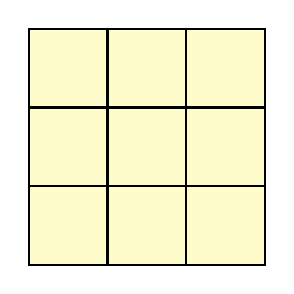
\begin{tikzpicture}
        \draw[thick,fill=yellow!20] (0,0) rectangle (3,3);
        \draw[thick] (1,0)--(1,3) (2,0)--(2,3) (0,1)--(3,1) (0,2)--(3,2);
    \end{tikzpicture}\par}
    \noindent Có tất cả \TTcham[1.5cm] hình vuông.
\end{bt}

\begin{center}
       \faGg\faGg\quad Hết Buổi 1 \quad\faGg\faGg
\end{center}

%%%%%%%%%%%%%%%%%%%%%%%%%%%%%%%%%%%%%%%%%%%%%%%%%%%%%%%%%%
%                       BUỔI 2  (90 phút)
%%%%%%%%%%%%%%%%%%%%%%%%%%%%%%%%%%%%%%%%%%%%%%%%%%%%%%%%%%
\newpage
\TTdatlaibai
\par\medskip
{\centering
        {\color{mauchinh!120}\bfseries\Large PHIẾU BÀI TẬP TOÁN TƯ DUY CẤP ĐỘ A}\\[3pt]
        {\color{mauchinh!120}\bfseries\Large CHỦ ĐỀ: ÔN TẬP BÀI TOÁN CÓ LỜI VĂN\\[2pt] PHÉP CỘNG, PHÉP TRỪ (BUỔI 2 - 90 PHÚT)}\par}
\vspace{6pt}
\TTthongtin

\TTgoiy{\textbf{Cách trình bày bài giải:} (1) Viết \textbf{tóm tắt}. (2) Viết \textbf{câu lời giải}. (3) Viết \textbf{phép tính} kèm đơn vị trong ngoặc. (4) Viết \textbf{đáp số}. \textit{Ví dụ:} Số quả cam có tất cả là: $38+25=63$ (quả). Đáp số: $63$ quả cam. \textbf{Chú ý:} ``nhiều hơn'', ``thêm'' thường là cộng; ``ít hơn'', ``còn lại'' thường là trừ, nhưng phải đọc kĩ đề vì có bài bị ``đánh lừa''!}

%---------------------------------------------------------
\TTphan{A}{CỦNG CỐ (khoảng 25 phút)}{1}

\begin{bt}
    Đọc tóm tắt rồi hoàn thành bài giải.
    \begin{listEX}
        \item Lan có $38$ nhãn vở, Hà có $25$ nhãn vở. Hỏi cả hai bạn có bao nhiêu nhãn vở?
        \TTtomtat{Lan: & $38$ nhãn vở}{Hà: & $25$ nhãn vở \quad Cả hai bạn: ? nhãn vở}
        \noindent\textbf{Bài giải}\par
        \noindent Số nhãn vở cả hai bạn có là:\par
        \noindent\hspace*{1.2cm}$38+25=\TTdien[0.8cm]$ (nhãn vở)\par
        \noindent\textbf{Đáp số:} \TTdien[0.8cm] nhãn vở.
        \item Mẹ có $71$ quả trứng, mẹ đã bán $36$ quả. Hỏi mẹ còn lại bao nhiêu quả trứng?
        \TTtomtat{Có: & $71$ quả trứng}{Đã bán: & $36$ quả trứng \quad Còn lại: ? quả trứng}
        \noindent\textbf{Bài giải}\par
        \noindent Số quả trứng mẹ còn lại là:\par
        \noindent\hspace*{1.2cm}\TTdien[0.8cm]$-$\TTdien[0.8cm]$=$\TTdien[0.8cm] (quả)\par
        \noindent\textbf{Đáp số:} \TTdien[0.8cm] quả trứng.
    \end{listEX}
\end{bt}

\begin{bt}
    Khoanh vào chữ cái đặt trước phép tính đúng để giải bài toán.
    \begin{listEX}
        \item Bao gạo nếp nặng $35$ kg. Bao gạo tẻ nặng hơn bao gạo nếp $12$ kg. Hỏi bao gạo tẻ nặng bao nhiêu ki-lô-gam?\par
        \textbf{A.} $35+12$ \hspace{1.2cm} \textbf{B.} $35-12$ \hspace{1.2cm} \textbf{C.} $35+35$
        \item Thùng thứ nhất có $62$ l dầu. Thùng thứ hai có ít hơn thùng thứ nhất $17$ l dầu. Hỏi thùng thứ hai có bao nhiêu lít dầu?\par
        \textbf{A.} $62+17$ \hspace{1.2cm} \textbf{B.} $62-17$ \hspace{1.2cm} \textbf{C.} $17-62$
    \end{listEX}
\end{bt}

\newpage
\begin{bt}
    Nối mỗi đề toán với phép tính dùng để giải bài toán đó.
    \TTbatdauhinh
    {\centering
    \begin{tikzpicture}[font=\small]
        \node[TTdeto] (a1) at (0,0) {Lan có $36$ viên bi, Hà có $27$ viên bi. Hỏi hai bạn có tất cả bao nhiêu viên bi?};
        \node[TTdeto] (a2) at (0,-1.4) {Cô có $50$ quả cam, cô cho đi $18$ quả. Hỏi cô còn lại bao nhiêu quả cam?};
        \node[TTdeto] (a3) at (0,-2.8) {Lan cho bạn $8$ quyển truyện thì còn lại $15$ quyển. Hỏi lúc đầu Lan có bao nhiêu quyển truyện?};
        \node[TTdeto] (a4) at (0,-4.2) {Bình có $45$ viên bi. An có ít hơn Bình $17$ viên bi. Hỏi An có bao nhiêu viên bi?};
        \foreach \k in {1,2,3,4}{\fill (a\k.east) ++(0.25,0) circle (2.5pt);}
        \node[TTpt] (b1) at (13.8,0) {$15+8$};
        \node[TTpt] (b2) at (13.8,-1.4) {$45-17$};
        \node[TTpt] (b3) at (13.8,-2.8) {$36+27$};
        \node[TTpt] (b4) at (13.8,-4.2) {$50-18$};
        \foreach \k in {1,2,3,4}{\fill (b\k.west) ++(-0.25,0) circle (2.5pt);}
    \end{tikzpicture}\par}
\end{bt}

\begin{bt}
    Nhìn sơ đồ đoạn thẳng, viết bài giải rồi tính.
    \TTbatdauhinh
    \noindent\begin{minipage}[t]{0.49\linewidth}\centering
        \begin{tikzpicture}[font=\sffamily\small,scale=0.95]
            \node[anchor=east] at (0,0.5) {Tổ 1};\node[anchor=east] at (0,-0.4) {Tổ 2};
            \draw[thick,fill=blue!10] (0.1,0.2) rectangle (3.1,0.8);\node at (1.6,0.5) {24 cây};
            \draw[thick,fill=blue!10] (0.1,-0.7) rectangle (3.1,-0.1);
            \draw[thick,fill=orange!30] (3.1,-0.7) rectangle (4.3,-0.1);\node at (3.7,-0.4) {9};
            \draw[decorate,decoration={brace,mirror,amplitude=4pt}] (0.1,-0.8)--(4.3,-0.8) node[midway,below=4pt] {?};
        \end{tikzpicture}\\[2pt]
        Tổ 1 trồng $24$ cây. Tổ 2 trồng nhiều hơn tổ 1 là $9$ cây. Hỏi tổ 2 trồng bao nhiêu cây?
    \end{minipage}\hfill
    \begin{minipage}[t]{0.49\linewidth}\centering
        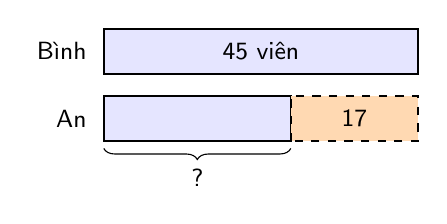
\begin{tikzpicture}[font=\sffamily\small,scale=0.95]
            \node[anchor=east] at (0,0.5) {Bình};\node[anchor=east] at (0,-0.4) {An};
            \draw[thick,fill=blue!10] (0.1,0.2) rectangle (4.3,0.8);\node at (2.2,0.5) {45 viên};
            \draw[thick,fill=blue!10] (0.1,-0.7) rectangle (2.6,-0.1);
            \draw[thick,dashed,fill=orange!30] (2.6,-0.7) rectangle (4.3,-0.1);\node at (3.45,-0.4) {17};
            \draw[decorate,decoration={brace,mirror,amplitude=4pt}] (0.1,-0.8)--(2.6,-0.8) node[midway,below=4pt] {?};
        \end{tikzpicture}\\[2pt]
        Bình có $45$ viên bi. An có ít hơn Bình $17$ viên bi. Hỏi An có bao nhiêu viên bi?
    \end{minipage}\par
    \begin{listEX}
        \item \TTgiai{1}
        \item \TTgiai{1}
    \end{listEX}
\end{bt}

%---------------------------------------------------------
\TTphan{B}{NÂNG CAO (khoảng 35 phút)}{2}

\begin{bt}
    Bạn Lan giải bài toán sau nhưng các bước bị xáo trộn. Em hãy sắp xếp lại cho đúng thứ tự.
    \par\smallskip\noindent\textbf{Đề:} Thùng thứ nhất có $35$ l nước. Thùng thứ hai có nhiều hơn thùng thứ nhất $12$ l nước. Hỏi cả hai thùng có bao nhiêu lít nước?
    \par\smallskip
    {\renewcommand{\arraystretch}{1.25}\noindent\begin{tabular}{@{\hspace{0.45cm}}l@{\ }l}
        \textbf{A.} & $35+47=82$ (l) \\
        \textbf{B.} & Số lít nước thùng thứ hai có là: \\
        \textbf{C.} & $35+12=47$ (l) \\
        \textbf{D.} & Số lít nước cả hai thùng có là: \\
        \textbf{E.} & Đáp số: $82$ l nước. \\
    \end{tabular}}
    \par\smallskip\noindent Thứ tự đúng là: \TTdien[0.8cm]\ $\to$\ \TTdien[0.8cm]\ $\to$\ \TTdien[0.8cm]\ $\to$\ \TTdien[0.8cm]\ $\to$\ \TTdien[0.8cm]
\end{bt}

\newpage
\begin{bt}
    Bạn Bình giải bài toán sau:
    \par\smallskip\noindent\textbf{Đề:} Nam có $30$ nhãn vở. Nam có ít hơn Mai $8$ nhãn vở. Hỏi Mai có bao nhiêu nhãn vở?
    \par\smallskip
    {\noindent\hspace*{0.45cm}\begin{tabular}{|l|}
        \hline
        \textbf{Bài giải} \\
        Số nhãn vở của Mai là: \\
        $30-8=22$ (nhãn vở) \\
        Đáp số: $22$ nhãn vở. \\
        \hline
    \end{tabular}}
    \begin{listEX}
        \item Bài giải của Bình đúng hay sai? \TTcham[2cm]
        \item Em hãy giải thích: ``Nam có \textbf{ít hơn} Mai'' thì ai có nhiều nhãn vở hơn? \TTcham[3cm]
        \item Em hãy giải lại cho đúng.
    \end{listEX}
    \TTgiai{1}
\end{bt}

\begin{bt}
    Tìm số lúc đầu.
    \begin{listEX}
        \item Lan có một số nhãn vở. Lan cho bạn $8$ nhãn vở thì còn lại $15$ nhãn vở. Hỏi lúc đầu Lan có bao nhiêu nhãn vở?
        \TTgiai{1}
        \item Trong giỏ có một số quả cam. Mẹ bỏ thêm $14$ quả cam thì trong giỏ có $50$ quả. Hỏi lúc đầu trong giỏ có bao nhiêu quả cam?
        \TTgiai{1}
    \end{listEX}
\end{bt}

\begin{bt}
    Trên xe buýt có $45$ người. Đến bến, có $18$ người xuống xe và $12$ người lên xe. Hỏi lúc này trên xe có bao nhiêu người?
    \TTgiai{2}
\end{bt}

\begin{bt}
    Bảng dưới đây cho biết số quyển sách bốn tổ trong lớp đã góp cho thư viện.
    \TTbatdauhinh
    {\centering
    \renewcommand{\arraystretch}{1.5}
    \begin{tabular}{|c|c|c|c|c|}
        \hline
        \textbf{Tổ} & Tổ 1 & Tổ 2 & Tổ 3 & Tổ 4 \\
        \hline
        \textbf{Số quyển sách} & 18 & 25 & 19 & 23 \\
        \hline
    \end{tabular}\par}
    \par\smallskip
    \begin{listEX}
        \item Tổ nào góp nhiều sách nhất? \TTcham[2cm]\hspace{0.5cm} Tổ nào góp ít sách nhất? \TTcham[2cm]
        \item Tổ góp nhiều sách nhất góp nhiều hơn tổ góp ít sách nhất bao nhiêu quyển?\par
        Phép tính: \TTcham[4cm] = \TTcham[2cm] (quyển)
        \item Tổ 3 và tổ 4 góp tất cả bao nhiêu quyển sách?\par
        Phép tính: \TTcham[4cm] = \TTcham[2cm] (quyển)
    \end{listEX}
\end{bt}

%---------------------------------------------------------
\TTphan{C}{THỬ THÁCH TƯ DUY - câu hỏi từ các kì thi Toán (khoảng 30 phút)}{3}

\begin{bt}
    \TTnguon{Dạng đề Olympic Toán - tính nhanh}
    Tính nhanh bằng cách ghép các số thích hợp.
    \TTgoiy{\textbf{Ví dụ:} $27+35+13=(27+13)+35=40+35=75$.}
    \begin{listEX}
        \item $25+38+15+12=\TTcham[2.5cm]$
        \item $64+28-28=\TTcham[2.5cm]$
        \item $50-18-2=\TTcham[2.5cm]$
        \item $11+12+13+14+15=\TTcham[2.5cm]$
    \end{listEX}
\end{bt}

\begin{bt}
    \TTnguon{Dạng đề Kangaroo - chữ số bị che}
    Mỗi ô vuông ẩn một chữ số. Em hãy tìm các chữ số đó.
    \par\smallskip
    {\centering
    $\begin{array}{r@{\ }c@{\ }c}
        & 4 & \TTdien[0.7cm] \\
        +\ & \TTdien[0.7cm] & 7 \\
        \hline
        & 9 & 1
    \end{array}$
    \hspace{3cm}
    $\begin{array}{r@{\ }c@{\ }c}
        & 8 & \TTdien[0.7cm] \\
        -\ & \TTdien[0.7cm] & 5 \\
        \hline
        & 4 & 8
    \end{array}$\par}
    \TTgoiy{\textbf{Gợi ý:} xét chữ số hàng đơn vị trước, nhớ xem phép tính có nhớ hay không.}
\end{bt}

\begin{bt}
    \TTnguon{Dạng đề SASMO - bài toán về tuổi}
    Anh hơn em $4$ tuổi. Tổng số tuổi của hai anh em là $12$ tuổi. Hỏi anh bao nhiêu tuổi, em bao nhiêu tuổi?
    \TTgoiy{\textbf{Gợi ý:} thử các tuổi của em rồi tính tuổi anh ($=$ tuổi em $+4$) và tổng hai tuổi.}
    \TTbatdauhinh
    {\centering
    \renewcommand{\arraystretch}{1.5}
    \begin{tabular}{|c|c|c|}
        \hline
        \textbf{Tuổi em} & \textbf{Tuổi anh} & \textbf{Tổng hai tuổi} \\
        \hline
        2 & 6 & 8 \\
        \hline
        3 & & \\
        \hline
        4 & & \\
        \hline
    \end{tabular}\par}
    \par\medskip\noindent Anh \TTcham[1.2cm] tuổi, em \TTcham[1.2cm] tuổi.
\end{bt}

\newpage
\begin{bt}
    \TTnguon{Dạng đề Toán Singapore - bài toán con ốc sên}
    Một con ốc sên bò lên một cái cột cao $8$ m. Ban ngày nó bò lên được $3$ m, ban đêm nó bị tụt xuống $1$ m. Hỏi sau mấy ngày thì con ốc sên lên tới đỉnh cột?
    \TTgoiy{\textbf{Gợi ý:} ghi lại độ cao của ốc sên sau mỗi buổi sáng và sau mỗi buổi tối. Chú ý: khi lên tới đỉnh cột thì ốc sên không còn bị tụt xuống nữa.}
    \TTbatdauhinh
    {\centering
    \renewcommand{\arraystretch}{1.5}
    \begin{tabular}{|c|c|c|}
        \hline
        \textbf{Ngày} & \textbf{Độ cao sau buổi sáng} & \textbf{Độ cao sau buổi tối} \\
        \hline
        Ngày 1 & 3 m & 2 m \\
        \hline
        Ngày 2 & \ \ \ \ \ \ \ \ \ \ \ \ & \ \ \ \ \ \ \ \ \ \ \ \ \\
        \hline
        Ngày 3 & & \\
        \hline
        Ngày 4 & & \\
        \hline
    \end{tabular}\par}
    \TTdapso
\end{bt}

\begin{bt}
    \TTnguon{Dạng đề Toán Singapore - nhiều hơn, ít hơn}
    An có nhiều hơn Bình $6$ viên bi. An cho Bình $2$ viên bi. Hỏi bây giờ ai có nhiều bi hơn và nhiều hơn bao nhiêu viên?
    \TTgoiy{\textbf{Gợi ý:} chọn một số bi cụ thể cho Bình (ví dụ $10$ viên), tính số bi của An, rồi cho bi và so sánh. Thử thêm một số khác để kiểm tra.}
    \TTbatdauhinh
    {\centering
    \renewcommand{\arraystretch}{1.5}
    \begin{tabular}{|c|c|c|c|c|}
        \hline
        & \multicolumn{2}{c|}{\textbf{Lúc đầu}} & \multicolumn{2}{c|}{\textbf{Sau khi An cho Bình 2 viên}} \\
        \hline
        & Bình & An & Bình & An \\
        \hline
        Thử 1 & 10 & 16 & & \\
        \hline
        Thử 2 & 20 & & & \\
        \hline
    \end{tabular}\par}
    \par\medskip\noindent Bây giờ \TTcham[1.5cm] có nhiều bi hơn, nhiều hơn \TTcham[1.2cm] viên bi.
\end{bt}

\begin{bt}
    \TTnguon{Dạng đề Violympic - xếp hàng}
    Các bạn học sinh xếp thành một hàng dọc. Mai đứng thứ $4$ tính từ đầu hàng và đứng thứ $5$ tính từ cuối hàng. Hỏi hàng đó có tất cả bao nhiêu bạn?
    \TTgoiy{\textbf{Gợi ý:} em hãy vẽ hàng bằng các chấm tròn, đánh dấu vị trí của Mai rồi đếm.}
    \par\smallskip\noindent\textbf{Em vẽ vào đây:}\par\vspace{1.4cm}
    \TTdapso
\end{bt}

\begin{center}
       \faGg\faGg\quad Hết Buổi 2 \quad\faGg\faGg
\end{center}
\end{document}
